% 09/11/2020 - First round of corrections: added Manolo's corrections
% 14/11/2020 - Second round of corrections: added Thomas (new) & Ray corrections
% 15/11/2020 - Grammarly

\begin{refsection}
%-------------------------------------------------------------------------
%-------------------------------------------------------------------------
\chapter{Modelling optical imperfections in refractive lenses}\label{sec:modelling}
%-------------------------------------------------------------------------
%-------------------------------------------------------------------------

To understand the impact of CRL on the optical design of complete beamlines, it is necessary to be able to simulate them realistically. The basic implementation of X-ray lenses is already available on the two most widespread beamline simulation tools: \textit{SHADOW} [\cite{SanchezdelRio2011}] and \textit{SRW} [\cite{Chubar1998}]. Both implementations, although based on different schemes, ray tracing [\cite{Alianelli2007}] and wave optics [\cite{Baltser2011}] respectively, are based on an ideal model combining refraction and absorption for the stacked lenses. Much has been done in terms of refining the modelling of ideal X-ray lenses [\cite{Umbach2008, SanchezdelRio2012, Osterhoff2013, Simons2017, Pedersen2018}] and, to a certain extent, the modelling of optical imperfections [\cite{Pantell2001, Andrejczuk2010, Gasilov2017, Osterhoff2017}]. Except for the work presented in [\cite{Roth2014}], investigating and simulating the inner structure of X-ray lenses, the present models consider mainly the lens shape and departure from a perfect parabolic shape. The majority of these models, however, is not publicly available, nor are readily compatible with standard beamline simulations suites like \textit{SHADOW} and \textit{SRW}. Another bottle-neck to the current literature or computer codes for simulating CRLs is that they do not include the data from real lens metrology, as is routinely done for X-ray mirrors simulations [\cite{SanchezDelRio2016}], which renders more difficult the inclusion of CRLs in simulations of complete beamline configurations in combination with other optical elements.

The modelling and functions presented here\footnote{This chapter is partially based on the work originally published in [\cite{Celestre2020b}].} are based on the framework of physical optics (cf. \S\ref{sec:physical_optics}~-~\textit{\nameref{sec:physical_optics}}) and are tailored to be used transparently with \textit{SRW} [\cite{Chubar1998}], which already provides a model for the CRL [\cite{Baltser2011}] - this basic ideal model combines refraction and absorption for the stacked lenses; optical imperfections from material inhomogeneities (voids, impurities) were later added [\cite{Roth2014}]. Expanding this model, we present the optical imperfections in refractive lenses in three different groups: \textit{i}-) misalignments of a single X-ray lens - Fig.~\ref{fig:lens_cuts}(b)-(c); \textit{ii}-) commonly encountered fabrication errors such as transverse offsets as well as tilts of the individual parabolic sections - Fig.~\ref{fig:lens_cuts}(d)-(g); \textit{iii}-) and other sources of deviations from the parabolic shape modelled with either polynomial decomposition of error functions or by using metrology data - Fig.~\ref{fig:metrology_zernike_profiles}. Each newly added feature is accompanied by a calculation of the residual thickness error, its impact on focusing by CRL and the beam caustic in the vicinity of the focal spot. The Strehl ratios for the different misalignments, fabrication errors and other sources of deviations from the parabolic profile are summarised in Fig.~\ref{fig:Strehl_m}. Calculations presented in this chapter are merely illustrative and a systematic evaluation is presented in \S\ref{sec:effect_optical_imperfections}~-~\textit{\nameref{sec:effect_optical_imperfections}}. All simulations shown throughout this chapter have similar conditions, that is, they model misalignments, fabrication errors or arbitrary residual errors of a single 2D-Beryllium lens with nominal radius $R=50~\mu\text{m}$, geometric aperture $A_{\diameter}=440~\mu\text{m}$ and $t_\text{wall}=20~\mu$m at 8~keV in fully-coherent simulations. The optical layout used for the simulations is shown in Fig.~\ref{fig:optical_layouts}. The code main functions implementing the ideal CRL and describing optical imperfections in refractive lenses are subsequently presented. The metrology technique used to measure the phase errors that arise from material inhomogeneities (voids, impurities) and/or figure errors from the lens forming process, namely, X-ray speckle tracking, is discussed in \S\ref{sec:measuring}~-~\textit{\nameref{sec:measuring}}.

\begin{figure}[t]
    \centering
    {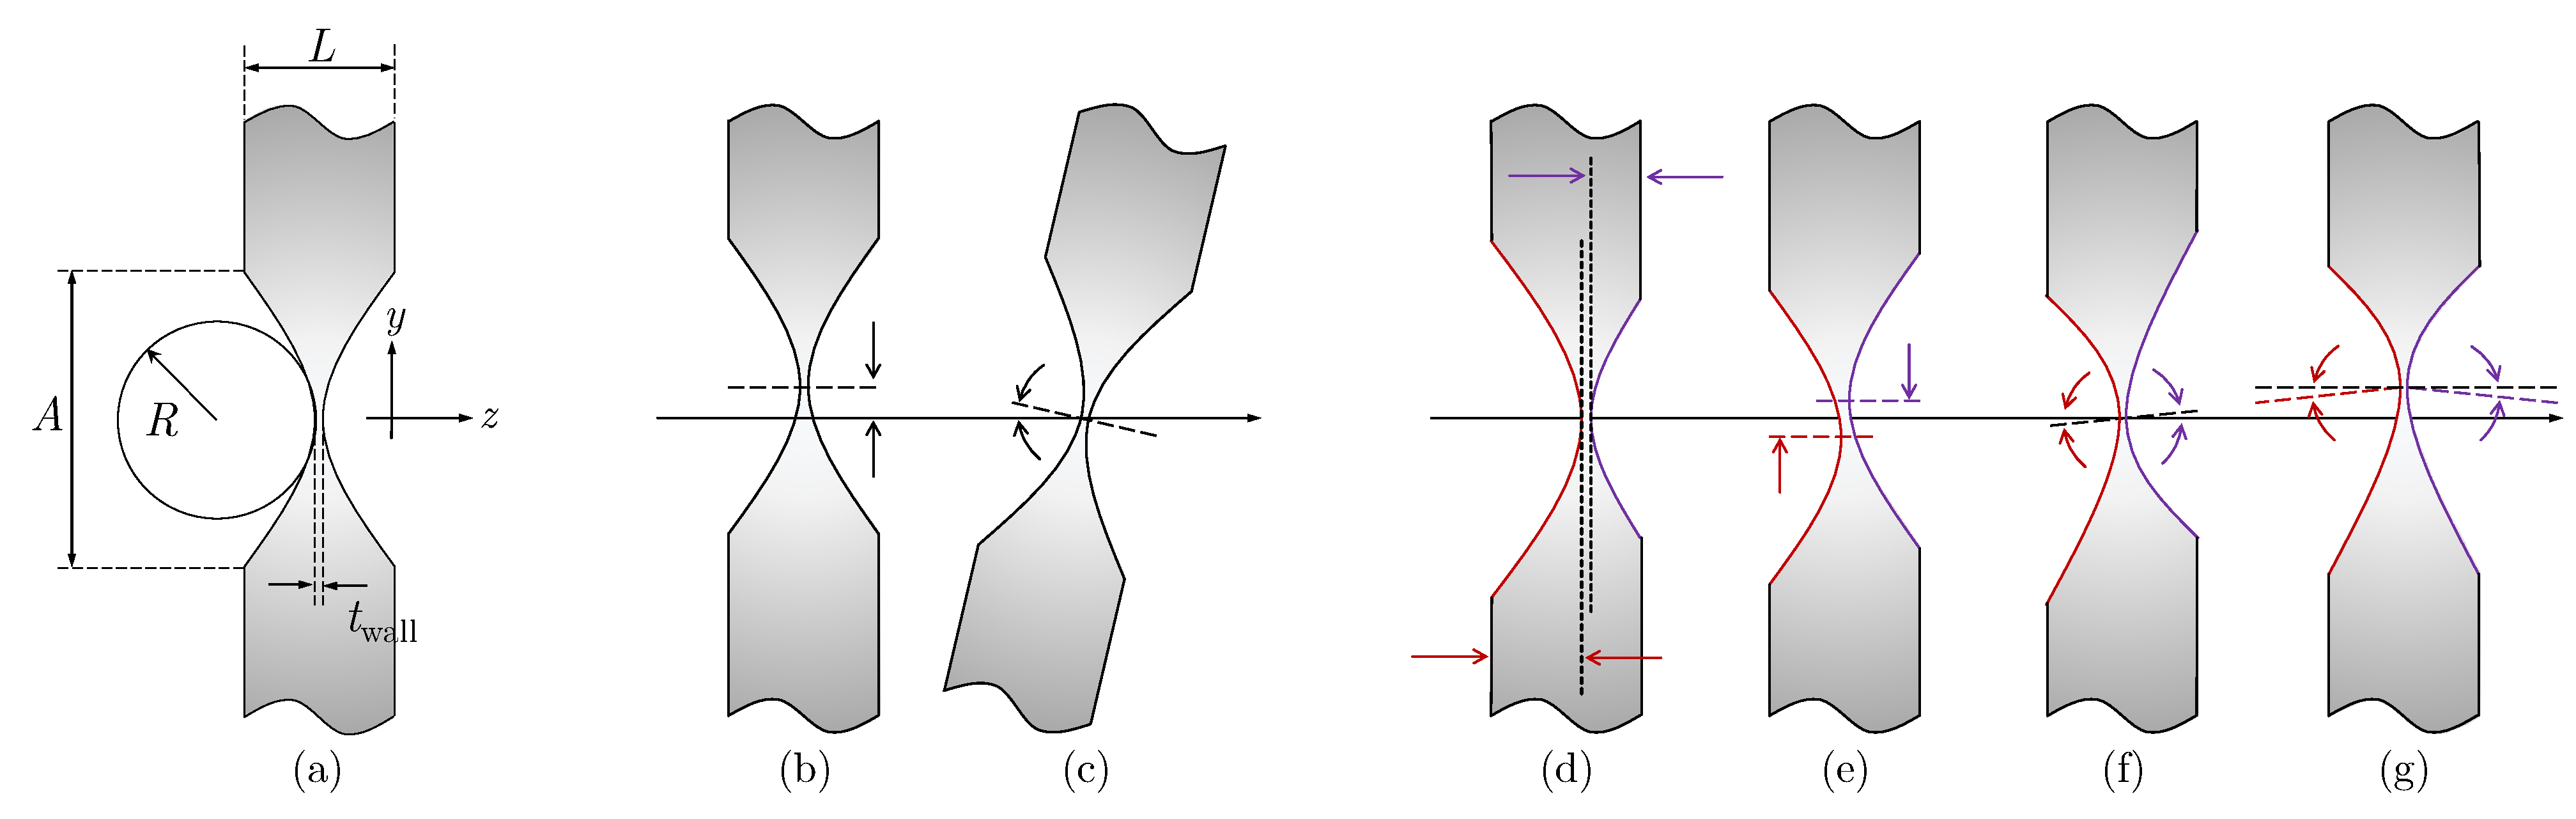
\includegraphics[width=0.9\linewidth]{figures/ch04/lens_cuts.pdf}}
    \caption[Modelling misalignments and fabrication errors in CRLs]{(a) ideal lens for reference. Lens typical misalignments are the (b) transverse offset and the (c) tilt or a combination of both. Common fabrication errors include the (d) longitudinal offset of the parabolic section, (e) transverse offset of the parabolic section and (f)-(g) tilted parabolic sections.}
    \label{fig:lens_cuts}
\end{figure}

%-------------------------------------------------------------------------
%-------------------------------------------------------------------------
\section{Optical imperfections in refractive lenses}\label{sec:describing_modelling}
%-------------------------------------------------------------------------
%-------------------------------------------------------------------------

In the paraxial approximation, the parabolic shape for a refracting surface is generally regarded as the ideal shape\footnote{The shape of a focusing refracting surface can be derived from the Fermat's principle, but the parabolic shape is generally regarded as a good approximation. Large apertures are often necessary when very small focused beams are required, but increasing the geometric aperture of the optical element causes the parabolic approximation to under-perform. Several aspheric surface shapes for different focusing conditions were reported in [\cite[Fig~4]{SanchezdelRio2012}]. For a deeper discussion on aspheric surfaces in the context of optics, please, refer to [\cite{Schulz1988}].} for minimising aberrations. It is legitimate, then, to define as errors any deviation from this ideal parabolic form\footnote{Such definition, however, leaves out discrepancies in the radius of curvature $R$ (designed vs. \textit{de facto}) and the associated defocus it may cause. Discrepancies between designed and executed lenses may render them to be labelled as out-of-specification and may cause the system to under-perform, but are not deviations of the parabolic shape, provided the ideal parabolic shape takes into account the \textit{de facto} radius of curvature. Accounting for such discrepancies can be done using the ideal model described by the transmission element $\mathrm{T}_{\text{single lens}}(\Delta_z)$ (cf. Eq.~\ref{eq:TE_singlelens}) using the \textit{de facto} radius of curvature.} regardless of their origin. The phase errors induced by an ideal lens misalignment will be presented first, then the typical fabrication errors of bi-concave lenses will be presented shortly after. The misalignment and fabrication errors presented in this section were derived from the accumulated experience in handling beryllium and aluminium bi-concave embossed lenses, which are the most available throughout beamlines in diverse synchrotron facilities. However, the modelling presented here is generic and can be applied to a wide-range of CRL from diverse fabrication processes\footnote{cf. Table~1 from the supplementary material relative to [\cite{Roth2017}].}.

The optical layouts used throughout this chapter for all simulations is shown in Fig.~\ref{fig:optical_layouts}. The emitted radiation is modelled by a filament-electron-beam passing through a CPMU18 undulator with 111 magnetic periods with $\Lambda=18$~mm on-axis magnetic period and magnetic field $B=0.9863~$T - cf. \S\ref{sec:brilliance}~-~\textit{\nameref{sec:brilliance}}. The electron-beam parameters are those corresponding to the ESRF-EBS upgrade [\cite{orangebook}]. An ideal parabolic phase-element with focal length $f=-60~$m is placed 60~m downstream the radiation source. This is done to give the illumination a plane phase - cf. Eq.~\ref{eq:planewave}. Immediately downstream the ideal lens, the X-ray lens being modelled is placed and any changes to the wave-field after it can be directly attributed to the model studied. A second ideal parabolic phase element can be placed downstream the probe to collimate the beam. This removal of the focusing phase term allows obtaining the residual phase, which can be used to recover a residual thickness error by using Eq.~\ref{eq:aux_funcs_transb}\footnote{Since the residual accumulated thickness translates directly into residual accumulated phase, both terms can be used interchangeably.}. The optical layout for phase-contrast image, beam-caustics and the PSF do not make use of this second ideal element. For reference and to allow subsequent comparison, Fig.~\ref{fig:ideal_CRL} shows the focusing of a single ideal 2D-beryllium lens with nominal radius $R=50~\mu\text{m}$, geometric aperture $A_{\diameter}=440~\mu\text{m}$ and $t_\text{wall}=20~\mu$m at 8~keV using the basic modelling described in Eq.~\ref{eq:TE_singlelens}.

\begin{figure}[t]
    \centering
    {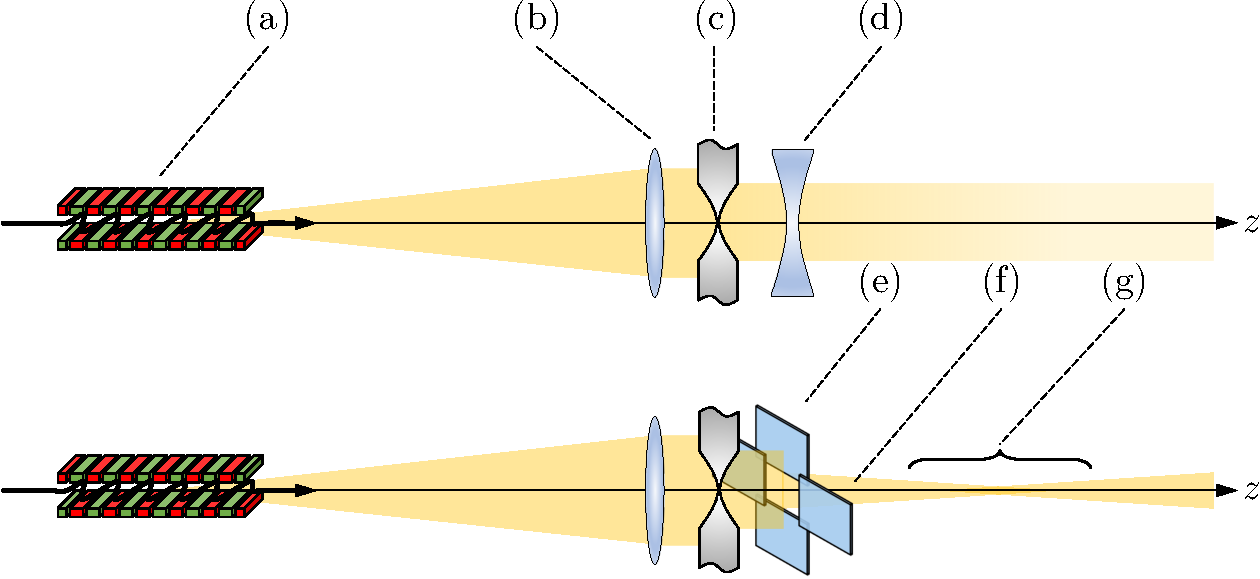
\includegraphics[width=.7\linewidth]{figures/ch04/simulations.pdf}}
    \caption[Optical layout used for modelling imperfections in CRL]{\textbf{top row}: optical setup used for calculating the residual phase and thickness. \textbf{bottom row}: setup for phase-contrast radiography, PSF and beam caustics. The illumination is from a filament electron beam passing through an undulator shown in (a). An (b) ideal parabolic phase element is placed to give the illumination a near-plane phase. Downstream of this ideal lens, the (c) X-ray lens is placed. An (d) ideal parabolic phase element can be placed downstream the probe in order to obtain the residual phase. Other measurements require other optical layouts. A (e) slit is put downstream the X-ray lens in order to contain the background and limit the beam to the lens geometric aperture. The phase-contrast image in can be obtained (f) downstream the lens and the beam-caustic range is shown in (g). At the centre of (g) the PSF is calculated.}
    \label{fig:optical_layouts}
\end{figure}
% \vspace{1cm}
 \begin{figure}[t]
        \centering
        % {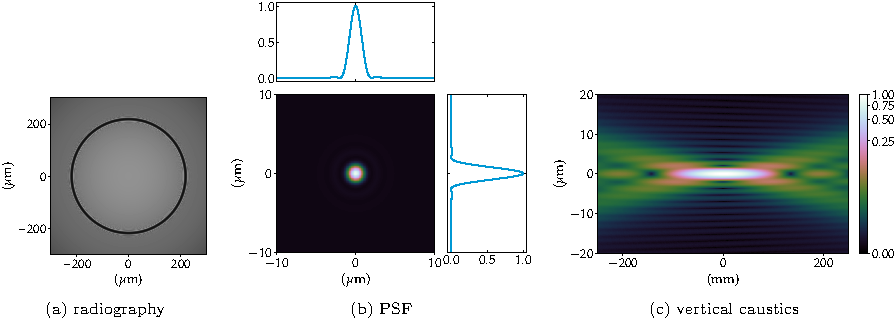
\includegraphics[height=4.19cm]{figures/ch04/CRL_ideal.pdf}}
        {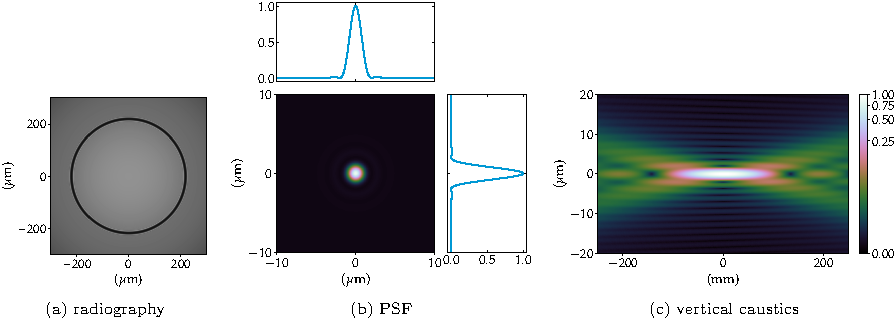
\includegraphics[height=4.19cm]{figures/compressed/CRL_ideal.pdf}}
        \caption[The ideal single X-ray lens]{Simulations of a single ideal 2D-beryllium lens with nominal radius $R=50~\mu\text{m}$, geometric aperture $A_{\diameter}=440~\mu\text{m}$ and $t_\text{wall}=20~\mu$m at $8$~keV  - cf. Fig~\ref{fig:lens_cuts}(a). (a) phase-contrast image $150~$mm downstream the ideal lens, (b) point-spread function with cuts centred in $(0,0)$ and (c) the vertical beam caustics from $-250$~mm to $250$~mm with respect to the focal plane at $f=4.701~$m.} \label{fig:ideal_CRL}
\end{figure}

%-------------------------------------------------------------------------
%-------------------------------------------------------------------------
\section{Misalignments}\label{sec:misalignments}
%-------------------------------------------------------------------------
%-------------------------------------------------------------------------

Misalignments of optical systems are not optical errors \textit{per se} as they can be mitigated by ensuring proper alignment is done; they will, however, cause changes to the ideal parabolic phase profile if left uncorrected and will affect the optical performance of the system. Although aligning a CRL stack is possible\footnote{The possibility of realignment of the CRL depends on where and how they are installed in the beamline. If their installation is on a bulky transfocator [\cite{Vaughan2011}], their realignment is more difficult to be performed. However, when used as a final focusing element, enclosed in small casings or compact transfocators - cf. Fig.~3 in [\cite{Lengeler1999}] and [\cite{Kornemann2017, Narikovich2019}], their realignment can be done more easily.}, the individual lenslets usually cannot be aligned to each other, hence the interest in modelling such misalignments.

%-------------------------------------------------------------------------
%-------------------------------------------------------------------------
\subsection{Transverse offset}\label{sec:trans_lens}
%-------------------------------------------------------------------------
%-------------------------------------------------------------------------

Displacing a single element a transverse distance $(\Delta_x,\Delta_y)$ can be simply done by calculating $\Delta_z(x-\Delta_x,y-\Delta_y)$ in Eq.~\ref{eq:ProjecThick}. The shifted element is depicted in Fig.~\ref{fig:lens_cuts}(b). For a pair of coordinates $(x,y)$:
\begin{equation}\label{eq:ProjecThick_misaligned}
    \Delta_z(x-\Delta_x,y-\Delta_y) = 
        \begin{cases}
      \cfrac{(x-\Delta_x)^2}{R_x}+\cfrac{(y-\Delta_y)^2}{R_y}+\text{t}_\text{wall}, &\quad\forall~(x-\Delta_x,y-\Delta_y) \in A,\\
      L, &\quad\text{otherwise}.
        \end{cases}
\end{equation}   
Eq.~\ref{eq:ProjecThick_misaligned} is the ideal parabolic profile of a bi-concave lens given by Eq.~\ref{eq:ProjecThick} with its vertices centred around $(\Delta_x,\Delta_y)$. While a single transversely shifted lens considered on its own is innocuous, piling up several shifted lenses has impacts on the overall accumulated phase parabolic shape and resulting geometric aperture. Although the exact effect of relative misalignments between individual lenses on the phase of the wave-field depends on the distance between lenslets, the energy, footprint and divergence of the X-ray beam, some insight can be gained by considering the individual focusing elements as thin-optical elements in intimate contact. Consider $N$ stacked lenses transversely misaligned with their transverse distance to the optical axis given by $(\Delta_{x_j},\Delta_{y_j})$, with $j=1,~2,~...,~N$. Within the intersection of their geometric apertures, the accumulated thickness is given by:
\begin{align}\label{eq:ProjecThick_Nmisaligned}
    \Delta_{z_\Sigma}(x,y) &= \sum\limits_{j=1}^N \Delta_z(\Delta_{x_j},\Delta_{y_j})\nonumber\\
    &=\sum\limits_{j=1}^N \underbrace{\frac{x^2}{R_{x_j}}+\frac{y^2}{R_{y_j}}}_\text{(I)}
    -\underbrace{2x\frac{\Delta_{x_j}}{R_{x_j}} - 2y\frac{\Delta_{y_j}}{R_{y_j}}}_\text{(II)}
    +\underbrace{\frac{\Delta_{x_j}^2}{R_{x_j}}+\frac{\Delta_{y_j}^2}{R_{y_j}}+\text{t}_{\text{wall}_j}}_\text{(III)}.
\end{align}
The first term in Eq.~\ref{eq:ProjecThick_Nmisaligned}, ($\text{I}$) is a quadratic term and it indicates ideal focusing as in Eq.~\ref{eq:ProjecThick}. The residual terms ($\text{II}$) and ($\text{III}$) are a linear term in $x$ and $y$ and a constant offset term, respectively. The first residual term, i.e. ($\text{II}$), adds a linear phase to the wave-front and acts like a prism, not deforming the monochromatic wave-field, but redirecting it. At the focal plane, the image position is transversely shifted but no change to the intensity and phase profiles is added. Symmetrically shifted lenses\footnote{That is $\Delta_{x_m}=-\Delta_{x_n}$ or $\Delta_{y_m}=-\Delta_{y_n}$ for $m,n\in(1,~2,~...,~N)$.} make ($\text{II}$) go to zero. The residual terms in ($\text{III}$) add a constant phase offset to the transmitted beam in addition to absorption. The effects of the transverse offset to a single X-ray lens are shown in Fig.~\ref{fig:shifted_CRL}.

\begin{figure}[t]
        \centering
        % {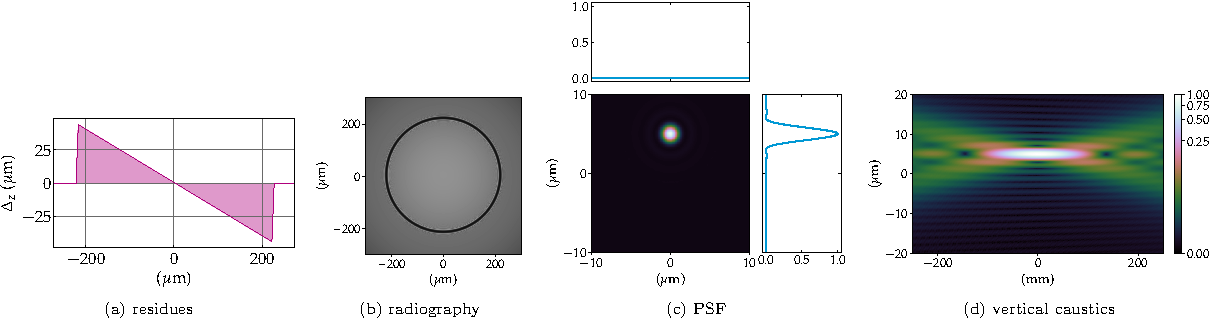
\includegraphics[height=4.19cm]{figures/ch04/shifted_CRL.pdf}}
        {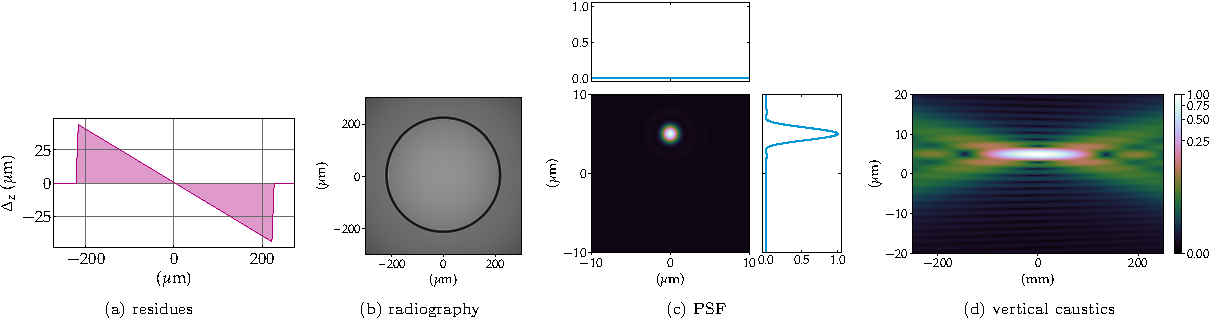
\includegraphics[height=4.19cm]{figures/compressed/shifted_CRL.pdf}}
        \caption[Effects of a transverse CRL offset]{Simulations of an ideal lens shifted by $\Delta_y=5~\mu$m - cf. Fig~\ref{fig:lens_cuts}(b). (a) Residual thickness, (b) phase-contrast image of the lens, (c) point spread function with cuts centred in $(0,0)$ and (c) the vertical beam caustics from $-250$~mm to $250$~mm with respect to the focal plane.} \label{fig:shifted_CRL}
\end{figure}

%-------------------------------------------------------------------------
%-------------------------------------------------------------------------
\subsection{Tilted lens}\label{sec:tilted_lens}
%-------------------------------------------------------------------------
%-------------------------------------------------------------------------

When rotating a lens in space as shown in Fig.~\ref{fig:lens_cuts}(c) and calculating its projected thickness, it is helpful to decouple the rotation of the front and back surfaces. This can be done by defining a point cloud in Cartesian coordinates:
\begin{subequations}\label{eq:point_cloud}
    \begin{align}
    z_\text{front surface}(x-\Delta_x,y-\Delta_y) &=\frac{\Delta_z(x-\Delta_x,y-\Delta_y)}{2},\\
    z_\text{back surface}(x-\Delta_x,y-\Delta_y) &= -\frac{\Delta_z(x-\Delta_x,y-\Delta_y)}{2}
    \end{align}
\end{subequations}{}
where $\Delta_z(x-\Delta_x,y-\Delta_y)$ is given by Eq.~\ref{eq:ProjecThick_misaligned}. The projected thickness is given by:
\begin{align}\label{eq:point_cloud_thickness}
    \Delta_z(x,y) = z_\text{front surface}(x,y) - z_\text{back surface}(x,y),
\end{align}{}
provided those are calculated on the same grid $(x,y)$. A tilted lens can be described by rotation matrices in three dimensions. In a system where the position is represented\footnote{Expressing the 3D coordinates as $(x,y,z,1)$ comes from homogeneous coordinates systems often used in projective geometry [\cite{House2016}].} as $(x,y,z,1)$ The transformation matrices allowing a rotation $\theta_{x,y,z}$ around each of the Cartesian axis are~[\cite{House2016}]:
\begin{align}\label{eq:affine}
    R_{\theta_x}= \begin{bmatrix}
                        1 & 0 & 0 &0\\
                        0 & c_x & -s_x  &0\\
                        0 & s_x & c_x &0\\
                        0 & 0 & 0 &1
    \end{bmatrix} ,\quad
    R_{\theta_y} = \begin{bmatrix}
                    c_y & 0 & s_y &0\\
                    0 & 1 & 0 &0\\
                    -s_y & 0 & c_y &0\\
                    0 & 0 & 0 &1
    \end{bmatrix}  ,\quad
    R_{\theta_z} = \begin{bmatrix}
                    c_z & -s_z & 0 &0\\
                    s_z & c_z & 0 &0\\
                    0 & 0 & 1 &0\\
                    0 & 0 & 0 &1
    \end{bmatrix},
\end{align}
where $c_\theta=\cos(\theta)$ and $s_\theta=\sin(\theta)$. $R_{\theta_x}$ denotes a rotation around the $x-$axis, $R_{\theta_y}$ around the $y-$axis and, finally, $R_{\theta_z}$ around the $z-$axis. Matrix multiplication is associative, which implies that if multiple rotations are involved, that is $R_{\theta_x}, R_{\theta_y}$ and $R_{\theta_z}$ are applied to a set of points $(x,y,z)$, an equivalent rotation matrix $R_{\theta}=R_{\theta_z}R_{\theta_y}R_{\theta_x}$ can be calculated and then, applied to those points is space: 
\begin{align}\label{eq:affine2}
    [x_\theta,y_\theta,z_\theta,1]^\text{T} & = R_{\theta_z}R_{\theta_y}R_{\theta_x}[x,y,z,1]^\text{T},\nonumber \\
     & = R_\theta[x,y,z,1]^\text{T},
\end{align}{}
where $(x_\theta,y_\theta,z_\theta)$ are the transformed $(x,y,z)$ coordinates after the $R_{\theta}=R_zR_yR_x$ rotation and the $^\text{T}$ in Eq.~\ref{eq:affine2} represents transposed matrices. The rotations given by $R_{\theta}$ have to be applied to both the front and back surfaces of the lens independently, with their respective point clouds given by Eqs.~\ref{eq:point_cloud}. In order to calculate the projected thickness along the optical axis, the rotated front and back surfaces have to be recalculated on a common grid, which is done by two-dimensional interpolation of $(x_\theta,y_\theta,z_\theta)$ to the original $(x,y)$ grid. The associative property allows for considerable computation time reduction, as the rotation can be done applying a single equivalent rotation matrix as opposed to three individual rotations. On the other hand, matrix multiplication is not commutative and the order of operations matter and should be specified\footnote{The implementation of the affine transformations for rotating CRLs in space follow the order: rotation around the $x-$axis ($R_x$), rotation around the $y-$axis ($R_y$) and then, rotation around the $z-$axis ($R_z$).}$^{,}$\footnote{For a deeper discussion on the properties of the affine transformations and coordinates systems, please refer to appendices \textit{C}-\textit{E} in [\cite{House2016}].} when rotating a point cloud. Equations~\ref{eq:affine} have their pivot point centred in the origin of their axis, that is, around $(x,y,z)=(0,0,0)$ in Cartesian coordinates. It is possible to define arbitrary pivot points with a combination of translations and rotations. Tilting an optical element in space will introduce aberrations to the beam propagation and its focusing\footnote{The interest in tilted optical elements and compensation is an active field, as evidenced by the literature on that subject - cf. [\cite{Guizar-Sicairos2011,Zhou2019,Ali2020}].}. This is apparent in the residual accumulated thickness in projection approximation shown in Fig.~\ref{fig:tilted_CRL}. The profile shown in Fig.~\ref{fig:tilted_CRL}(a) is proportional to the 4$^{\text{th}}$ power of the lateral coordinates in the direction of the shift. This contributes for the elongation of the beam along the propagation direction and shift on the focal plane position as shown in Fig.~\ref{fig:tilted_CRL}(d), which is a typical sign of spherical aberrations. It is also possible to see how the two surfaces (back and front) do not overlap, causing a slight reduction in the geometric aperture area, which gives rise to the the discontinuities in Fig.~\ref{fig:tilted_CRL}(a).

\begin{figure}[t]
        \centering
        % {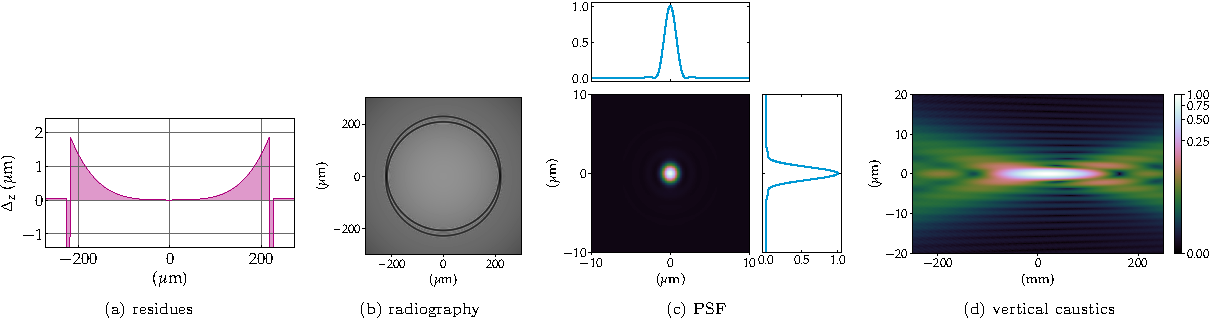
\includegraphics[height=4.19cm]{figures/ch04/tilted_CRL.pdf}}
        {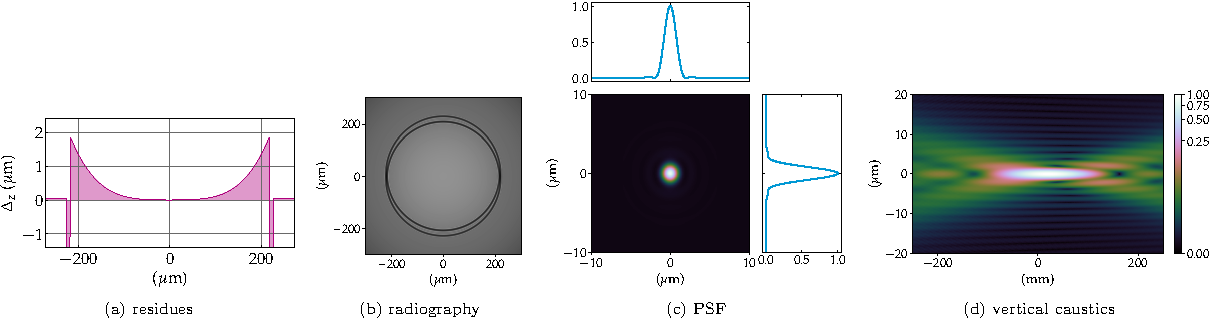
\includegraphics[height=4.19cm]{figures/compressed/tilted_CRL.pdf}}
        \caption[Effects of a CRL tilt]{Simulations of an ideal lens tilted by $\theta_x=1^{\circ}$ - cf. Fig~\ref{fig:lens_cuts}(c). (a) Residual thickness, (b) phase-contrast image of the lens, (c) point spread function with cuts centred in $(0,0)$ and (c) the vertical beam caustics from $-250$~mm to $250$~mm with respect to the focal plane. } \label{fig:tilted_CRL}
\end{figure}
%-------------------------------------------------------------------------
%-------------------------------------------------------------------------
\section{Fabrication errors}\label{sec:fabrication}
%-------------------------------------------------------------------------
%-------------------------------------------------------------------------

Modelling the typical misalignment of X-ray lenses implies calculating the lateral displacements and rotations in space of an ideal X-ray lens. However, bi-concave lenses may also present misalignments between the front and back focusing surfaces, which are closely related to the manufacturing processes involved in the lens production. Here, the front and back focusing surfaces are treated independently, allowing to model longitudinal and transverse misalignments as well as tilts of the front and back focusing surface concerning the optical axis.

%-------------------------------------------------------------------------
%-------------------------------------------------------------------------
\subsection{Longitudinal offset of the parabolic section}
%-------------------------------------------------------------------------
%-------------------------------------------------------------------------

Longitudinal offsets of the parabolic portions of a bi-concave X-ray lens appear when, for the same radius of curvature $R$, one parabolic portion reaches deeper into the lens disc than the other one - cf. Fig.~\ref{fig:lens_cuts}(d). The first eminent observation is that front and back surfaces will have different geometric apertures along the focusing direction. The new geometric aperture of the longitudinally offset parabolic profile can be calculated as:
\begin{equation}\label{eq:A_2}
    A_{\text{offset}} = 2\sqrt{[L-(\text{t}_\text{wall}+2\cdot\text{offset})]R},
\end{equation}{}
where a positive offset increases the apparent web thickness of the half lens to $\text{t}_\text{wall}/2+\text{offset}$ and decreases the geometric aperture for a fixed lens thickness. The aperture given by $A_{\text{offset}}$ and the apparent web thickness are used in Eq.~\ref{eq:point_cloud_thickness} (cf. Eqs.~\ref{eq:ProjecThick_misaligned} and \ref{eq:point_cloud}) when calculating the projected thickness.
Longitudinal offsets do not affect the parabolic accumulated shape of a single lens within $A_{\text{offset}}$ and, consequently, do not impose any optical imperfection to an optical system based on such lenses. However, they are often encountered in real lenses\footnote{Especially in embossed lenses, where different penetration depths of the punches often lead to asymmetric lenses.} and merit the implementation in the lens modelling. Fig.~\ref{fig:longitudinal_offset} shows the simulated profile and a radiography of a real lens showing the effects of the longitudinal offset of the parabolic section.

\begin{figure}[t]
        \centering
        % {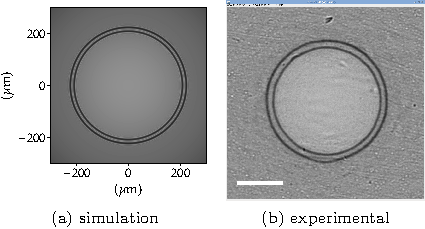
\includegraphics[height=3.cm]{figures/ch04/longitudinal_offset.pdf}}
        {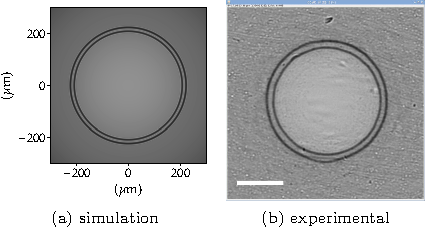
\includegraphics[height=3.cm]{figures/compressed/longitudinal_offset.pdf}}
        \caption[Effects of the longitudinal offset of the parabolic section]{(a) Simulated and (b) measured phase-contrast image of a single of a 2D-beryllium lens with nominal radius $R=50~\mu\text{m}$ with designed geometric aperture $A_{\diameter}=440~\mu\text{m}$. The scale bar in (b) is $200~\mu$m wide.} \label{fig:longitudinal_offset}
\end{figure}

%-------------------------------------------------------------------------
%-------------------------------------------------------------------------
\subsection{Transverse offset of the parabolic section}
%-------------------------------------------------------------------------
%-------------------------------------------------------------------------

Although parallel to the optical axis, it is possible that the parabolic surfaces axes are not collinear. This is shown in Fig.~\ref{fig:lens_cuts}(e). The modelling of the transverse offset of the front or/and back surfaces of a lens concerning the optical axis is done by calculating the net offset of each surface, that is the sum of lens transverse offset with the front or/and back surface transverse offset, and applying it to Eqs.~\ref{eq:point_cloud} when calculating Eq.~\ref{eq:point_cloud_thickness}. The effects on the residual accumulated phase of non-collinear parabolic surfaces are the same as the one described in the section \S\ref{sec:trans_lens}~-~\textit{\nameref{sec:trans_lens}}, that is, the presence in the residual phase of a linear and a constant term, which can be seen in Fig.~\ref{fig:offset_fs_CRL}.


\begin{figure}[t]
        \centering
        % 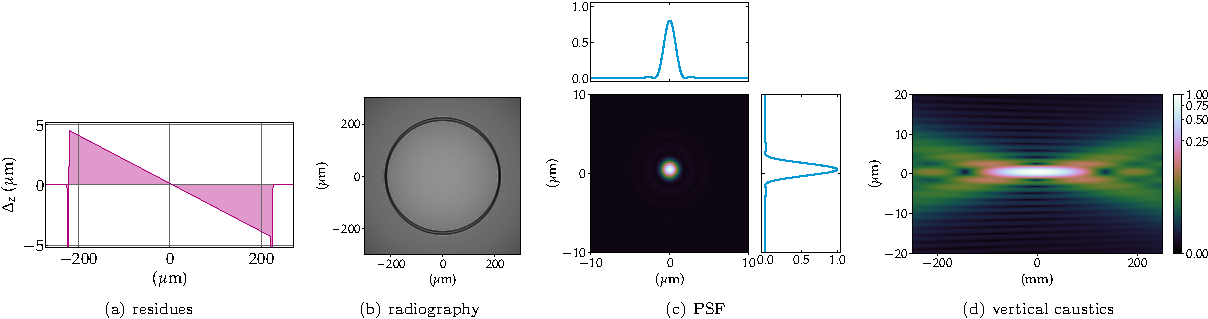
\includegraphics[height=4.19cm]{figures/ch04/offset_fs_CRL.pdf}
        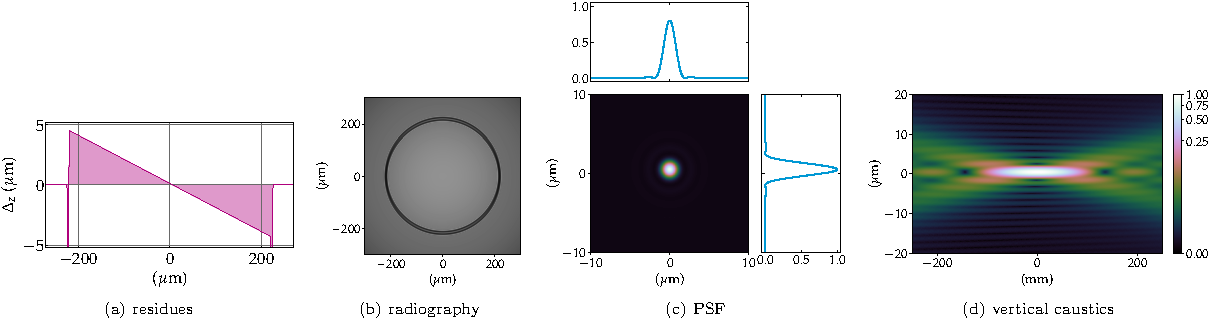
\includegraphics[height=4.19cm]{figures/compressed/offset_fs_CRL.pdf}
        \caption[Effects of the transverse offset of the parabolic section]{Simulations of a lens with front focusing parabolic section shifted by $\Delta_y=-2~\mu$m and back focusing shifted by $\Delta_y=-3~\mu$m - cf. Fig~\ref{fig:lens_cuts}(e). (a) Residual thickness, (b) phase-contrast image of the lens, (c) point spread function with cuts centred in $(0,0)$ and (c) the vertical beam caustics.} \label{fig:offset_fs_CRL}
\end{figure}

%-------------------------------------------------------------------------
%-------------------------------------------------------------------------
\subsection{Tilted parabolic section}
%-------------------------------------------------------------------------
%-------------------------------------------------------------------------

When the axes of the parabolic front or/and back surfaces are not parallel to the optical axis, the lens active area appears to be tilted as shown in Figs.~\ref{fig:lens_cuts}(f)~and~(g). Similarly to what was introduced in the section \S\ref{sec:tilted_lens}~-~\textit{\nameref{sec:tilted_lens}}, both front and back surfaces are rotated according to the rotation matrices described in Eqs.~\ref{eq:affine} and the procedure described by Eq.~\ref{eq:affine2}. There are two subtle differences: the rotation angles from front and back surfaces can be chosen independently and the rotation is only applied to the curved part of the lens, and not to the whole front and back surfaces including the flat parts. The independent rotations allow for different regimes: one where both imprints are tilted with the same angle as in shown in Fig.~\ref{fig:lens_cuts}(f), which yields a residual phase similar to the one discussed in \S\ref{sec:tilted_lens}~-~\textit{\nameref{sec:tilted_lens}}; and one where front and back surfaces are tilted with different angles, which yields an asymmetric residual phase as shown in Fig.~\ref{fig:tilt_fs_CRL}. By not applying the rotation to the plane region the lens projected thickness $L$ is not changed. A close inspection of Fig.~\ref{fig:tilt_fs_CRL} shows that while the symmetric case has a residual phase proportional to the 4$^{\text{th}}$ power of the lateral coordinates in the direction of the tilt, elongating the beam focusing in the propagation direction and shifting it on the same direction - typical of spherical aberrations, the residual phase of the anti-symmetric case has residual phase proportional to the 3$^{\text{rd}}$ power of the lateral coordinates in the direction of the tilt and has a PSF typical of coma-aberrated systems. The behaviour of the anti-symmetric case resulting in coma aberrations is commonly encountered in tilted one-sided kinoform lenses and zone-plates as reported in [\cite{Guizar-Sicairos2011,Ali2020}]. 

\begin{figure}[t]
        \centering
        % {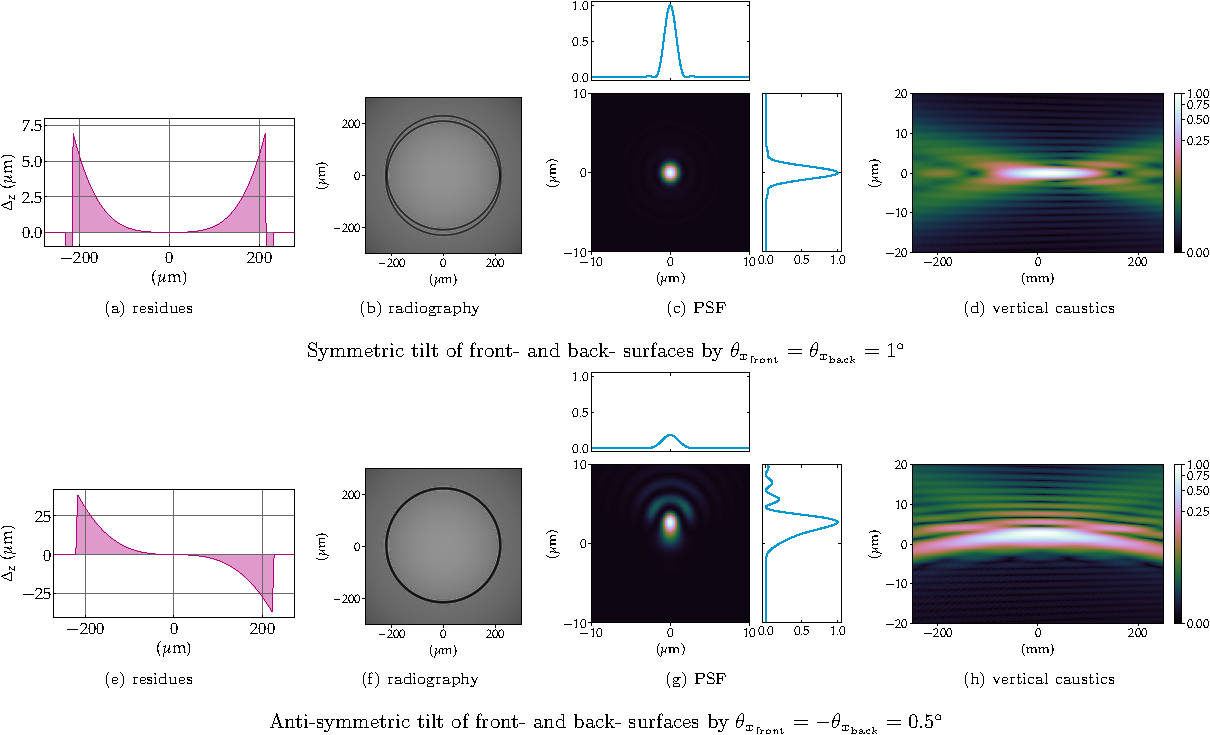
\includegraphics[width=1.\linewidth]{figures/ch04/tilt_fs_CRL.pdf}}
        {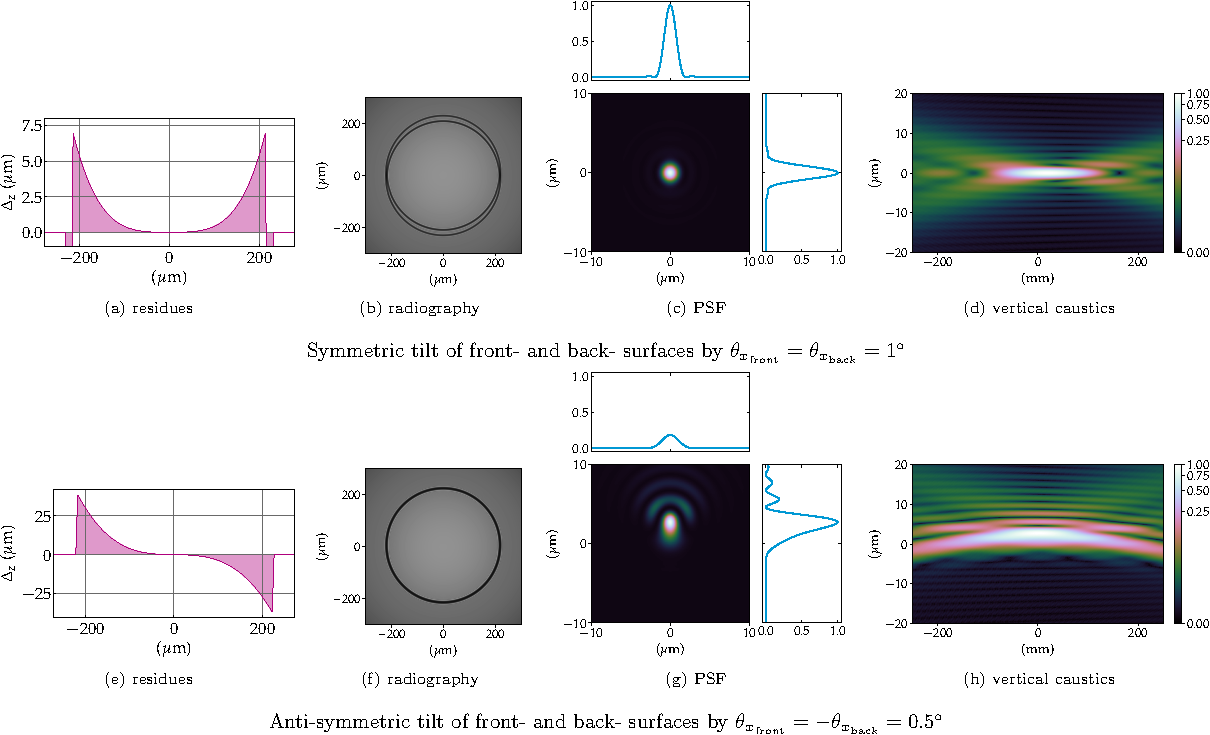
\includegraphics[width=1.\linewidth]{figures/compressed/tilt_fs_CRL.pdf}}
        \caption[Effects of the tilted parabolic section]{Simulations of a lens with front and back focusing parabolic sections independently tilted as shown in Fig~\ref{fig:lens_cuts}(f) and (g). The (a) residual thickness, (b) phase-contrast image, (c) point spread function and (c) the vertical beam caustics of the symmetric tilt are shown on the top row. The (e) residual thickness, (f) phase-contrast image, (g) point spread function and (h) the vertical beam caustics for the anty-symmetric case with the same conditions is presented in the bottom row.} \label{fig:tilt_fs_CRL}
\end{figure}
%-------------------------------------------------------------------------
%-------------------------------------------------------------------------
\section{Other sources of deviations from the parabolic shape}\label{sec:other_sources}
%-------------------------------------------------------------------------
%-------------------------------------------------------------------------

So far, the modelling described here relies on translations and rotations of an ideal parabolic surface and investigating the residual phase. Another equally valid approach is to manipulate directly the residual phase and add it to the phase of an ideal focusing lens, which can be done fitting arbitrary surfaces or by introducing data from metrology of the optical element to be simulated.

\begin{figure}[t]
        \centering
        {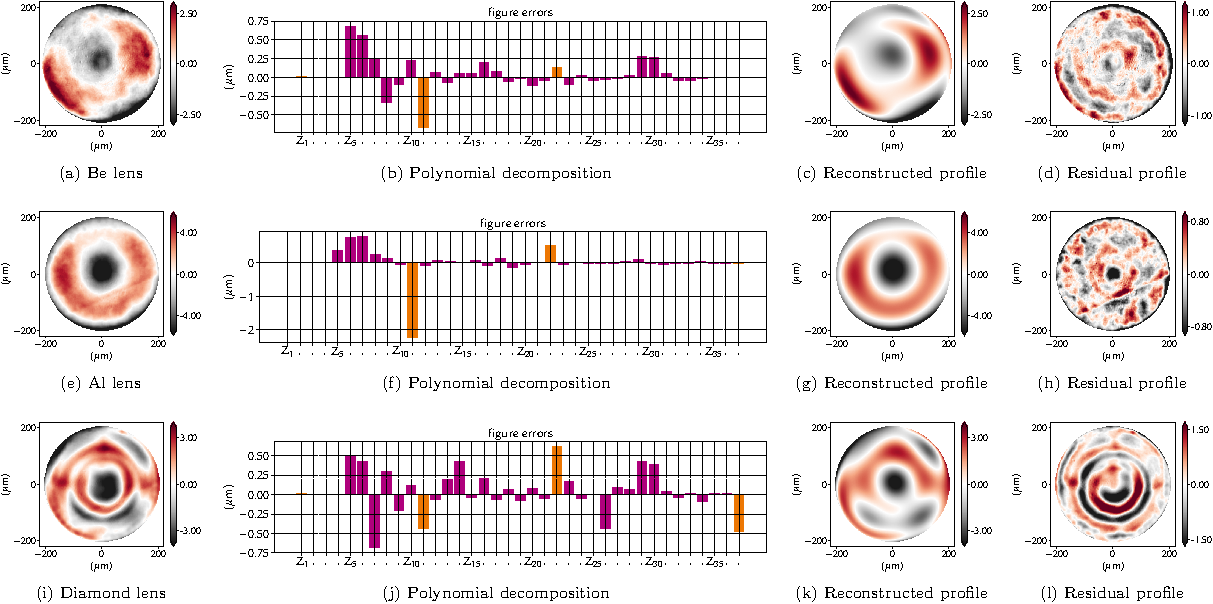
\includegraphics[width=1.\linewidth]{figures/ch04/metrology_zernike_profiles.pdf}}
        \caption[Other sources of deviations from the parabolic shape]{Comparison of the decomposition of errors in Zernike circle polynomials for beryllium, aluminium and diamond 2D lenses. \textbf{First row}: Be lens with (a) projected profile with RMS value $\sigma_z=1.4~\mu$m; (b) polynomial decomposition of the profile in (a); (c) the reconstruction based on those coefficients with RMS value $\sigma_z=1.3~\mu$m; and (d) the residual profile after the fit. \textbf{Middle row}: Al lens (e) projected profile with RMS value $\sigma_z=2.6~\mu$m; (f) polynomial decomposition of the profile in (e); (g) the reconstruction based on those coefficients with RMS value $\sigma_z=2.5~\mu$m; and (h) the residual profile after the fit. \textbf{Bottom row}: diamond lens with (i) projected profile with RMS value $\sigma_z=1.8~\mu$m; (j) polynomial decomposition of the profile in (i); (k) the reconstruction based on those coefficients with RMS value: $\sigma_z=1.6~\mu$m; and (d) the residual profile after the fit.}
        \label{fig:metrology_zernike_profiles}
\end{figure}

\begin{figure}[t]
        \centering
        {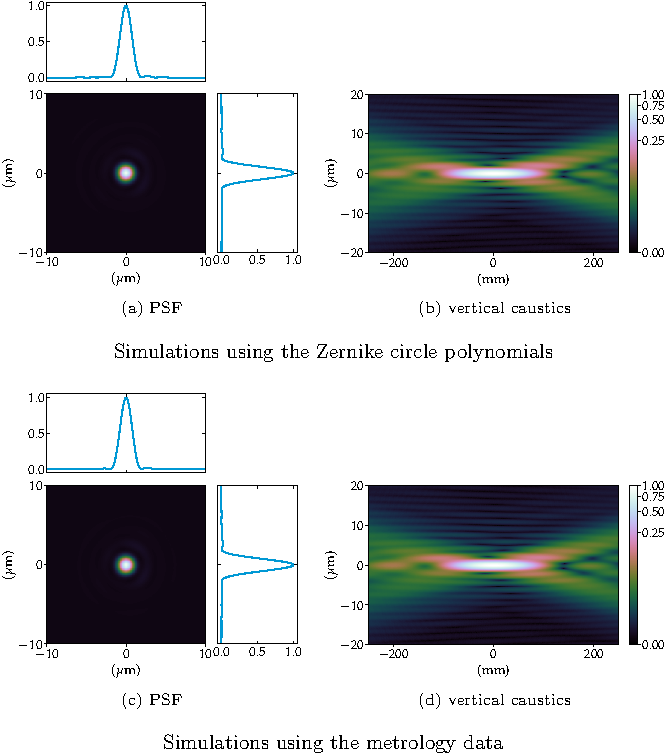
\includegraphics[height=10cm]{figures/ch04/metrology_zernike_simualtions.pdf}}
        \caption[Effects of other sources of deviations from the parabolic shape - single lens]{Simulations of a single 2D-beryllium lens with nominal radius $R=50~\mu\text{m}$, geometric aperture $A_{\diameter}=440~\mu\text{m}$ and $t_\text{wall}=20~\mu$m at 8~keV. \textbf{top row}: (a) metrology profile, (b) point-spread function with cuts centred in $(0,0)$ and (c) vertical beam caustics from -250~mm to 250~mm with respect to the focal plane. \textbf{bottom row}: (d) profile generated by the Zernike circle polynomials coefficients, (e) PSF and (f) beam caustics.} \label{fig:metrology_zernike_simualtions}
\end{figure}

\begin{figure}[t]
        \centering
        {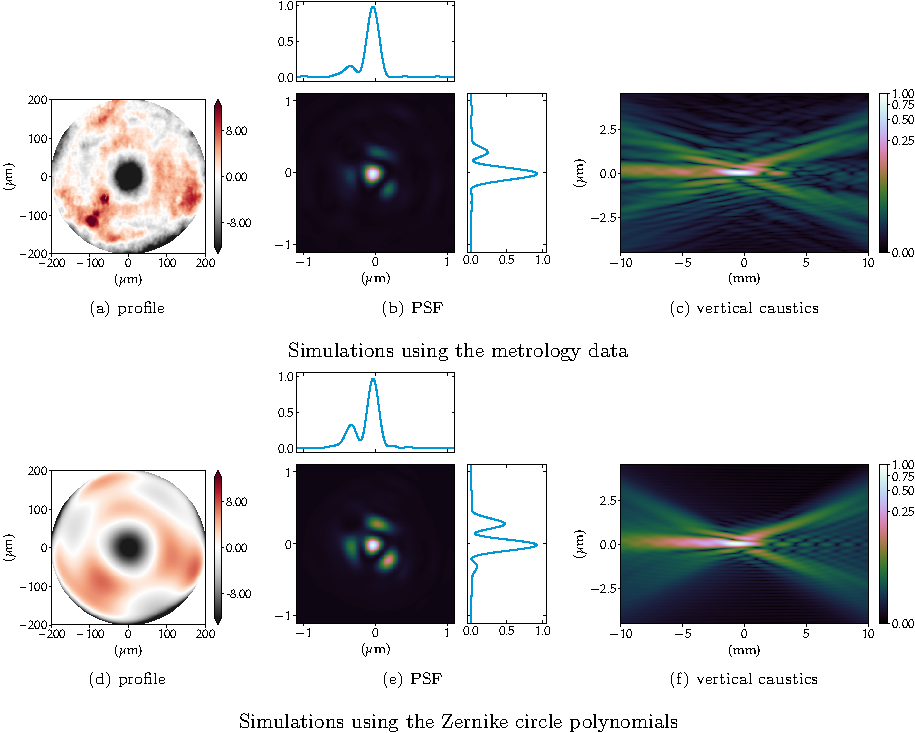
\includegraphics[height=10cm]{figures/ch04/metrology_zernike_simualtionsb.pdf}}
        \caption[Effects of other sources of deviations from the parabolic shape - 10-lens stack]{Simulations of 10 stacked 2D-beryllium lenses with nominal radius $R=50~\mu\text{m}$, geometric aperture $A_{\diameter}=440~\mu\text{m}$ and $t_\text{wall}=20~\mu$m at 8~keV. \textbf{top row}: (a) metrology profile, (b) point-spread function with cuts centred in $(0,0)$ and (c) vertical beam caustics from -10~mm to 10~mm with respect to the focal plane. \textbf{bottom row}: (d) profile generated by the Zernike circle polynomials coefficients, (e) PSF and (f) beam caustics.} \label{fig:metrology_zernike_simualtionsb}
\end{figure}

%-------------------------------------------------------------------------
%-------------------------------------------------------------------------
\subsection{Orthornormal polynomials}\label{sec:orthonormal_polynomials}
%-------------------------------------------------------------------------
%-------------------------------------------------------------------------

A widespread form of representing optical aberrations of arbitrary shapes is by decomposing them into an orthonormal base. Perhaps the most ubiquitous set of aberration functions is given by the Zernike polynomials for a circular aperture, first described in [\cite{Zernike1934}]. Their appeal comes from the fact that not only they are directly related to Seidel (primary), Schwarzschild (secondary) and tertiary-aberrations\footnote{This jargon comes from a power-series expansion of the aberration function. There are five primary aberrations, nine secondary aberrations and fourteen aberration terms for the tertiary aberrations. They all involve spherical aberration, coma, astigmatism, field curvature, distortion and variations of thereof [\cite{Mahajan2013}].} but also include piston and tilts; they form an orthonormal base, which means that the value of the coefficients is not affected by the removal of a particular term [\cite{Mahajan2007}]. Another advantage of the Zernike polynomial decomposition is that each orthonormal aberration coefficient is the standard deviation for that particular aberration over the exit pupil, which is valuable when evaluating the optical system compliance with the  Mar\'echal criteria and calculating the Strehl ratio [\cite{Mahajan1983}].

For the aforementioned decomposition of the aberration function in an orthonormal base to retain its properties, the application of the circular Zernike polynomials must be limited to circular apertures. Other shapes of apertures with- or without obscuration can be obtained by Gram-Schmidt orthonormalisation and weighting of the Zernike circle polynomials [\cite{Swantner1994,Mahajan1995}]. X-ray optics systems often have a rectangular aperture and two sets of polynomials are of particular interest in optical design: the set of orthonormal Zernike polynomials for a rectangular aperture  [\cite{Mahajan2007, Mahajan2012}] and the 2D-Legendre polynomial set for a rectangular aperture [\cite{Mahajan2010}]. Preferentially\footnote{Prof. V. Mahajan (University of Arizona, USA) and Prof. H. Gross (University of Jena, Germany) are acknowledged for discussions on orthonormal polynomials in wavefront analysis and pointing out relevant literature.}, the Zernike circle polynomials are applied to 2D focusing lenses with a circular aperture. For 2D focusing X-ray lenses with square aperture, low aspect ratio between horizontal and vertical apertures and not strongly astigmatic focusing, e.g. crossed planar X-ray lenses, the Zernike rectangular polynomials are preferred. The 1D focusing lens is better fit by the 2D Legendre polynomial set\footnote{Please, refer to [\cite{Ye2014}] for a comparison between 2D orthonormal sets for square apertures.}. Analysing and describing refractive X-ray optics using circular Zernike and 2D Legendre polynomials were first presented by [\cite{Koch2016}]. 

Fitting a surface to a given set of orthonormal polynomials is very useful as it allows to characterise and classify optical systems based on the types of aberrations it presents, which can be useful when mitigation strategies are being drawn (balancing aberrations). In addition to that, surfaces mimicking optical can be generated by asserting coefficients to a given polynomial set. This can be used to understand and isolate the effects of a given type of aberration or be used to represent a real surface when the coefficients for a particular optical element are known. Profiles generated by Zernike circle polynomials are shown in Fig.~\ref{fig:metrology_zernike_profiles}. They were generated using coefficients obtained from metrology data. The fit profiles resemble the metrology profiles they are based on - cf. left-hand side of Fig.~\ref{fig:metrology_zernike_profiles}. A comparison between the effects on a coherent X-ray beam for both profiles is shown in Fig.~\ref{fig:metrology_zernike_simualtions}. The difference between both simulation sets is almost imperceivable, whuch can be explained by the similarity between both figure error profiles and the fact that the difference between the figure errors RMS value is almost negligible: $\sigma_z=1.3~\mu$m (Zernike polynomial reconstruction) against $\sigma_z=1.4~\mu$m (metrology data), while the Mar\'echal criterion calculated for beryllium lenses illuminated at $8$~keV requires the accumulated projected figure errors to be $\sigma_z\leq2.08~\mu$m, which makes the impact in the reduction in intensity at the focal position is almost negligible - cf. Eqs.~\ref{eq:Strehl}-\ref{eq:ThickLim} for the Mar\'echal criteria and Strehl ratio in \textit{Tolerance conditions for aberrations} from \S\ref{sec:CRL_performance}~-~\textit{\nameref{sec:CRL_performance}}. Fig.~\ref{fig:metrology_zernike_simualtionsb} shows the same kind of comparison in Fig.~\ref{fig:metrology_zernike_profiles}, but with a less similar fit fit. Simulations still show good agreements, showing the same features: side-lobes (typical of trefoil aberration), elongated tail upstream the focal plane and 'Y'-shaped profile cut downstream.

%-------------------------------------------------------------------------
%-------------------------------------------------------------------------
\subsection{Metrology data}\label{sec:metrology_data}
%-------------------------------------------------------------------------
%-------------------------------------------------------------------------

Any (unintentional) deviation from the parabolic shape can be considered as a manufacturing error. Each manufacturing process has some type of (signature) error associated to it and with the increasing number of exotic - or unconventional - designs and tailored manufacturing strategies, it is unreasonable to create a model that could parametrise all sources of deviations from the parabolic shape. To circumvent that and to accurately model phase imperfections in compound refractive lenses, metrology data can also be used for optically imperfect X-ray lenses [\cite{Celestre2020, Chubar2020}]. Fig.~\ref{fig:metrology_zernike_profiles} shows three examples of lens figure errors from (a)-(d) a commercial pressed beryllium lens, (e)-(h) an in-house pressed aluminium lens and a (i)-(l) in-development laser-ablated diamond lens from a commercial partner. The figure errors were measured with at-wavelength metrology\footnote{cf. \S\ref{sec:at_wavelength}~-~\textit{\nameref{sec:at_wavelength}}.} and can be directly plugged into simulations [\cite{Celestre2020}]. The effects of optical imperfections from metrology data on a coherent X-ray beam are shown in Fig.~\ref{fig:metrology_zernike_simualtions} and Fig.~\ref{fig:metrology_zernike_simualtionsb}. The systematic use of metrology data for modelling optical imperfections in compound refractive lenses is explored in depth in \S\ref{sec:effect_optical_imperfections}~-~\textit{\nameref{sec:effect_optical_imperfections}}. The chapter \S\ref{sec:corrections}~-~\textit{\nameref{sec:corrections}} exemplifies how the framework developed to model such experimentally determined phase errors also opens the avenue to calculating the effects of any arbitrary phase modifying element.

\begin{figure}[t]
        \centering
        {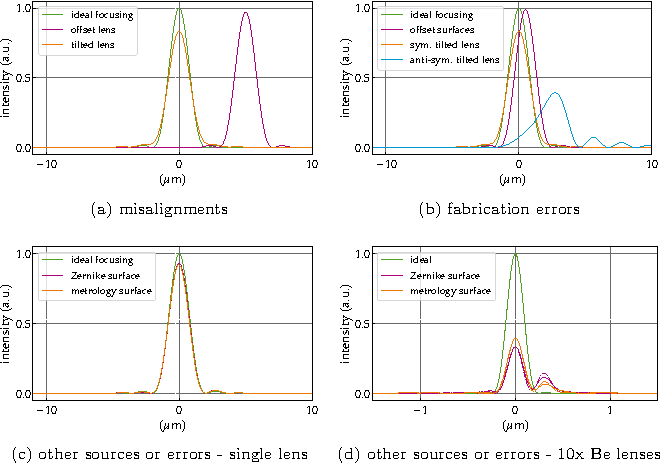
\includegraphics[width=0.75\linewidth]{figures/ch04/Strehl}}
        \caption[Strehl ratio summarising the results from the diverse models presented]{Strehl ratio of the vertical cut at $x=0$ summarising the results from the diverse models presented.} \label{fig:Strehl_m}
\end{figure}
%-------------------------------------------------------------------------
%-------------------------------------------------------------------------
\section{Implementation}
%-------------------------------------------------------------------------
%-------------------------------------------------------------------------

The implementation of the modelling of X-ray lenses with their typical misalignments, fabrication errors and other sources of optical imperfections is presented in the Python library \href{https://gitlab.esrf.fr/celestre/barc4RefractiveOptics}{\texttt{barc4RefractiveOptics}}, available on GitLab\footnote{\url{https://gitlab.esrf.fr/celestre/barc4RefractiveOptics}}$^,$\footnote{An OASYS (OrAnge SYnchrotron Suite) distribution to be used with \textit{SRW}, \textit{SHADOW} and \textit{SHADOW}-hybrid mode is being prepared. For updates on that, please, refer to the project GitHub page: \url{https://github.com/oasys-kit/oasys-barc4ro}. The OASYS implementation of \texttt{barc4RefractiveOptics} is being lead by Luca Rebuffi (Argonne National Lab. USA).} under a CC BY-SA 4.0 license, where more information on the implemented functions can be found. This library contains three main modules, namely: \texttt{projected\_thickness.py}, \texttt{wavefront\_fitting.py} and \texttt{barc4RefractiveOptics.py}.

The module \texttt{projected\_thickness.py} is responsible for the calculation of the thickness in projection approximation for the ideal lens (Eq.~\ref{eq:TE_singlelens}); lenses with the misalignments discussed in \S\ref{sec:misalignments}~-~\textit{\nameref{sec:misalignments}}; with the fabrication errors presented in \S\ref{sec:fabrication}~-~\textit{\nameref{sec:fabrication}}; and other sources of deviations from the parabolic profile described in \S\ref{sec:orthonormal_polynomials}~-~\textit{\nameref{sec:orthonormal_polynomials}}, which are based on Zernike (circular and rectangular) polynomials or the 2D Legendre polynomials\footnote{The functions used to generate the 2D circular Zernike polynomials contain pieces of codes from the module \texttt{libtim-py} from Tim van Werkhoven, that had to be brought to Python 3.7 and in some places, small bugs had to be fixed - this module has a Creative Commons Attribution-Share Alike
license. The 2D rectangular Zernike was originally inspired by the analytical formulation from the module \texttt{opticspy} from Xing Fan, which has an MIT license. The formulation from the module was based on the equations from [\cite{Mahajan2007}], but had to be corrected with the errata published in [\cite{Mahajan2012}]. The 2D Legendre polynomials were implemented based on the formulations in [\cite{Mahajan2010}]. A lot of effort was done in bringing all these three distinct libraries into a homogeneous and concise module.}. To generate an arbitrary profile the user can either use a list with the coefficients or enter an RMS value for their sum, in which case, the coefficients will be randomly calculated and will add up to the RMS value limited by the user input. The fit of a wavefront to a set of orthonormal polynomials is a very important diagnostic tool for optical modelling and is available within the \texttt{wavefront\_fitting.py} module, which currently supports the Zerkine circle and rectangular as well as the 2D Legendre polynomial sets.

The modules just described generate 2D projected thickness maps and in conjunction with the metrology data (2D height profiles) are interfaced to \textit{SRW}\footnote{Available at \url{https://github.com/ochubar/srw}} by \texttt{barc4RefractiveOptics.py}. This module is written to be used transparently with the optical element class \texttt{SRWLOpt} described in the module \texttt{srwlib.py} from \textit{SRW}. Each function representing either an X-ray lens or its figure errors returns a class \texttt{SRWLOptT} representing a generic transmission element storing amplitude transmission and optical path difference as a function of transverse coordinates. The main calculations for generating the X-ray lens transmission element is performed by the function \texttt{srwl\_opt\_setup\_CRL}. The generation of the residual phase errors based on the polynomial expansion of the aberration function in the exit pupil is done by \texttt{srwl\_opt\_setup\_CRL\_errors}. This function is used in conjunction with \texttt{srwl\_opt\_setup\_CRL} as modelled in Eq.~\ref{eq:TE_CRL_single_ERR}. The generation of a surface based on the metrology data is done by \texttt{srwl\_opt\_setup\_CRL\_metrology}. The metrology data should be saved as an ASCII file (.dat) as defined by the function \texttt{srwl\_uti\_save\_intens\_ascii} from the module \texttt{srwlib.py}. The function \texttt{srwl\_opt\_setup\_CRL\_metrology} can be used to simulate figure errors, in which case, much like \texttt{srwl\_opt\_setup\_CRL\_errors} it requires the use of \texttt{srwl\_opt\_setup\_CRL} or it can be used to simulate a full measured profile. 

Separating the calculation of the projected thickness $\Delta_z$ from the interface to SRW allows the module \texttt{projected\_thickness.py} to be used in any X-ray optical simulation code based on physical optics as the transmission elements can be directly calculated from the 2D surface maps by using the Eq.~\ref{eq:transmission_operator}. $\blacksquare$

% %-------------------------------------------------------------------------

\addcontentsline{toc}{section}{References}
\printbibliography[heading=subbibliography]
\end{refsection}

